\documentclass{ijclclp}
\usepackage{subcaption}

% This template is intanted to be used with the XeLaTex compiler for supporting CJK fonts
% Title Information
\title{Surface simplification}
\author{Jakob Drusany and Yon Ploj}

% Document Start
\begin{document}

\maketitle
% Abstract Section
\begin{abstract}
In this project, we implement an algorithm that iteratively reduces the triangle count of a triangulated surface while preserving its overall structure as accurately as possible.
\end{abstract}

% Sections
\section{Introduction}
Surface simplification is a common necessity across various fields that work with surfaces. It serves multiple purposes, such as reducing the complexity of the mesh to enhance computational efficiency, smoothing the measurement noise from sources such as 3D scanners, analyzing features at different resolutions, and more.

To achieve this, we implemented the \textit{edge contraction algorithm}
which in each iteration removes an edge $ab$ and replaces it with an optimal point $c$ to reduce deformation. This can only be done if the topological type of the surface is preserved by the operation.
\section{Theoretical background}
In this section, the simplified theory behind the algorithm is presented.
\subsection{Edge contraction}
\begin{figure}[h]
    \centering
    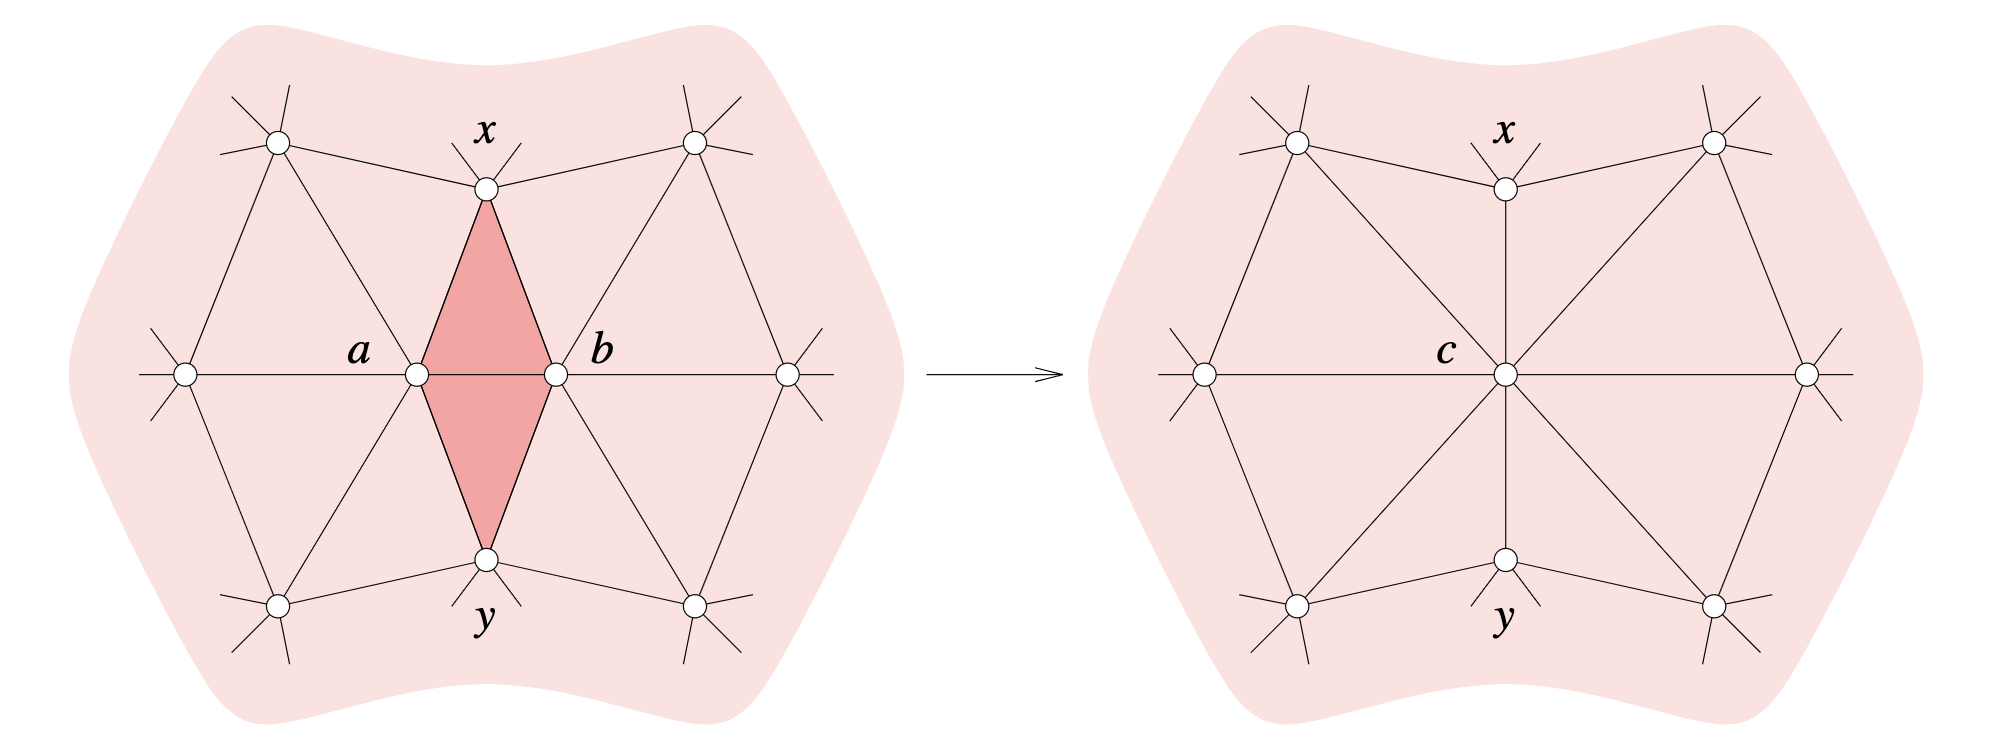
\includegraphics[width=0.8\linewidth]{contraction.png}
    \caption{The contraction of $ab$ removes the 2 dark triangles and glues the two left edges to the two right edges}
    \label{fig:contraction}
\end{figure}
Suppose $K$ is a triangulation of a 2-manifold without boundary. Let $a$ and $b$ be two vertices and $ab$ the connecting edge in $K$. We define the \textit{contraction} operation as the operation that identifies $a$ with $b$ and removes all newly generated duplicates. If we call the new vertex $c$, we can get the new triangulation $L$ from $K$ by:
\begin{itemize}
    \item removing $ab$, $abx$, $aby$
    \item replacing all occurrences of $a$ and $b$ with $c$
    \item removing potential duplicates in $L$
\end{itemize}

\subsection{Preserving the shape}
If we want to talk about shape, we have to embed $K$ into $\mathbb{R}^3$ with straight edges and flat triangles. We will define an error function that will tell us how much an edge contraction deforms the shape. To do this, we must look at the planes spanned by the triangles adjacent to the edge $ab$. The deformation depends on where we place the new vertex $c$. To find the optimal position of $c$, we have to find the point that has the smallest sum of squared distances to all planes spanned by the triangles adjacent to $ab$. We call this sum $E_H(x)$ where $x$ is a proposed position of $c$ and $H$ is a finite set of planes. A plane $h$ is defined by a unit normal $u \in \mathbb{R}^3, |u|=1$ and an offset $\delta \in \mathbb{R}$. The plane is then the set of points $y \in \mathbb{R}^3$ for which $y \cdot u = -\delta$ holds. The signed distance of a point $x\in \mathbb{R}^3$ is then $d(x,h) = x^T \cdot u + \delta$. If we define $x'^T = (x^T, 1)$ and $u'^T = (u^T, \delta)$ we can simplify the expression into a simple four-dimensional scalar product $d(x,h) = x'^T \cdot u'$. Now, the sum of the squared distance from a set of planes $H$ is just $E_H(x) = \sum_{h_i \in H} d^2(x, h_i)$.
\[E_H(x) = \sum_{h_i \in H} d^2(x, h_i) = \sum_{h_i \in H} (x'^T \cdot u_i')(u_i'^T \cdot x') = x'^T \cdot \left( \sum_{h_i \in H} u_i' \cdot u_i'^T \right) \cdot x'\]
We can rewrite this expression as $E_H(x) = x^T \cdot Q \cdot x$ where \[Q = \sum_{h_i \in H} u_i' \cdot u_i'^T\]
Each set of planes $H$ has a unique symmetric four-by-four matrix, to which we refer as the \textit{fundamental matrix}.

The function $E_H(x)$ depends on a proposed location $x$ and a set of planes $H$ that are obtained from a certain edge $ab$. So, the function depends on $ab$ and $x$. If we want to compute the error of contracting an edge, we need a function that depends only on a given edge, so we define the function $Error$ as the minimum $E_H(c)$ on all possible placements of $c$.
\[Error(ab) = \min_{c \in \mathbb{R}^3}E_H(c).\]

We can compute this by first obtaining the $Q$ matrix and then solving a simple system of equations
\[x'Q[i] = 0 \text{ for } i=1,2,3\]
where $Q[i]$ represents the $i$-th column of $Q$. The system is underdetermined, as we have 3 equations and 4 variables, so we can always find a solution where the fourth element of $x'$ is non-zero. We need this because if we want to obtain the 3-coordinates of $x$, we need to write $x'^T$ in the form $(x^T, 1)$.

\subsection{The algorithm}
Now that we know how an edge contraction is computed, we have to choose which edge to contract. We will iteratively contract edges, on each step choosing the one that results in the least amount of error. To achieve this, we calculate the $Error(ab)$ for each edge and insert them into a priority queue, where the edges with the smaller errors are on top.
Then we can define the main loop:
\begin{verbatim}
while not empty(queue) do ab = min_element(queue);
    if is_safe(ab) then contract(ab) endif
endwhile
\end{verbatim}
The function \texttt{is\_safe} determines if removing the edge $ab$ preserves the topological type. To compute this, we define the link of an edge an vertex:
\[\text{Lk} ab = \{x \in K\ |\ abx \in K\}\]
\[\text{Lk} a = \{x,xy \in K\ |\ ax,axy \in K\}\]
and use the link condition lemma which states that the triangulations $K$ and $L$ have the same topological type $\iff$ Lk$ab$ = Lk$a\ \cap$ Lk$b$.

\subsection{Optimisation}
The main benefit of the $Q$-matrix is that we do not have to compute the matrix for each edge for every step, but we can maintain it throughout the algorithm. When we contract an edge $ab$, we have to compute the $Q$-matrix of the new vertex $H_c = H_a \cup H_b$. This is not a disjoint set, so we can not just add the respective $Q$-matrices. Instead, we have to use inclusion-exclusion and subtract the intersection $H_ab = H_a \cap H_b$ which is stored from the previous steps.

So at the beginning, we compute and store the quadratics for all triangles, edges, and verices. For a triangle $abx$ we compute $Q_{abx}$. For an edge $ab$, we compute $Q_{ab} = Q_{abx} + Q_{aby}$ because the edge $ab$ is adjacent to triangles $abx$ and $aby$. For a vertex $a$ we compute $Q_a$ as the sum of all the quadratics of triangles that are adjacent to $a$.
After each contraction, we compute the quadratic of the new vertex $Q_c = Q_a + Q_b - Q_{ab}$ and the two new edges $Q_{cx} = Q_{ax} + Q_{bx} - Q_{abx}$ and $Q_{cy} = Q_{ay} + Q_{by} - Q_{aby}$.
\newpage
\section{Implementation}
We implemented the algorithm in \textit{julia}, it takes in a \textit{.ply} file (Stanford Triangle Format) and outputs a video of how the mesh contracts through time. The algorithm works only on 2-dimensional closed manifolds (surfaces), so some preprocessing may be required (e.g. closing holes).

We have 2 main data structures, one is \texttt{SimplicialComplex2D} which holds all of the triangles, edges, and vertices. The edges and vertices are stored in neighbourhood arrays (\texttt{\_vertex\_to\_edges} stores all edges adjacent to a certain point and \texttt{\_edge\_to\_triangles} stores all triangles connected to a certain edge). The \texttt{ContractedSimplicialComplex2D} stores the contracted simplex and all of its $Q$ matrices.

The main loop is in \texttt{main.jl} which loads the object, calls the preprocessing function, fills the holes, and then starts the main loop. The main loop iterates with a priority queue of edges for contraction and creates a video of the contraction. Because the contractions happen logarithmically (at the start not much happens, at the end the object is contracted very fast), we visualise the object every time \texttt{100*log(vertex\_count)} changes.
The preprocessing happens in \texttt{preprocessing.jl} which fills the holes and uses a KDTree to mitigate the  coordinate mismatch in adjacent triangles due to floating point inaccuracies. The code for contraction, fundamental quadratics calculation, and issafe is in \texttt{contractions.jl}. Because our triangles are stored sorted by vertex index, we lose the orientation of the triangles. This presents a problem in the visualisation of the mesh because the normals are not consistent. This is solved in \texttt{visualisations.jl} which contains the code for orienting the surface and drawing it.
\newpage
\section{Results}
We have confirmed that the original and the contracted homologies are the same. The algorithm was tested on a few meshes:
\begin{itemize}
\item The "Stanford Bunny" - The Stanford 3D Scanning Repository
\begin{figure}[h]
\centering
\begin{subfigure}{.4\textwidth}
  \centering
  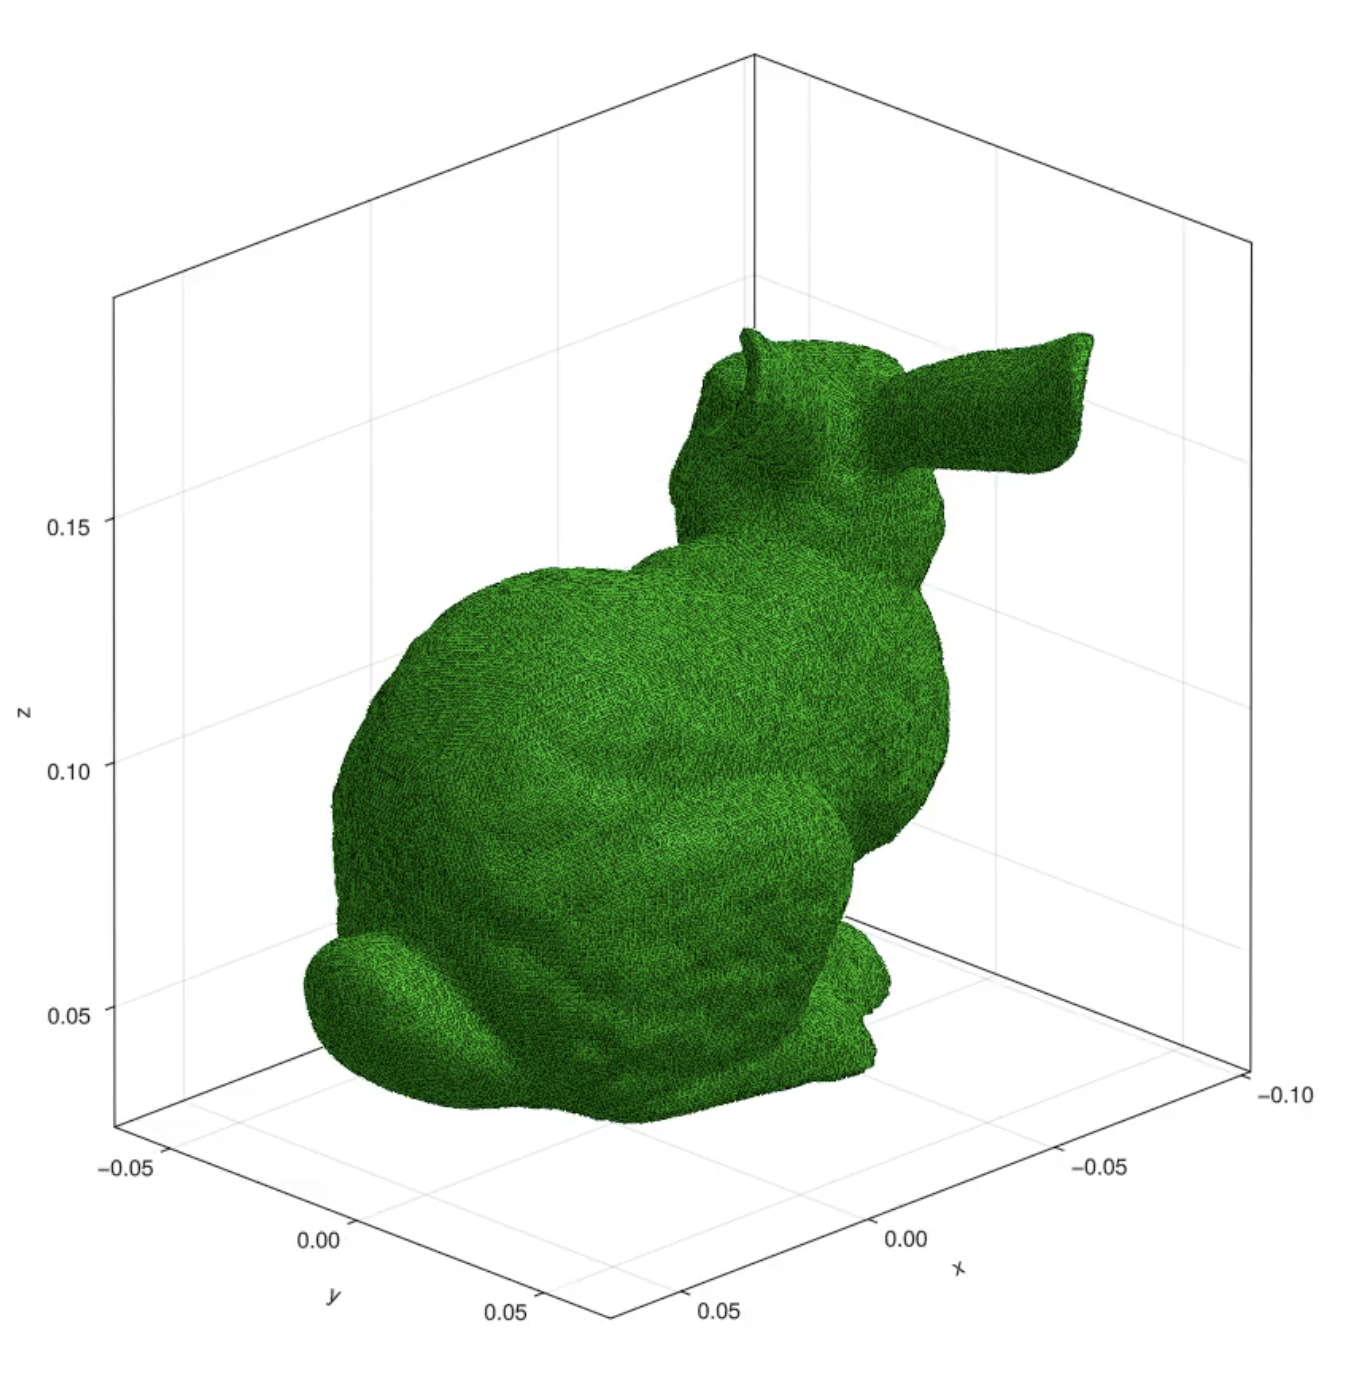
\includegraphics[width=\linewidth]{buni1.png}
\end{subfigure}
\begin{subfigure}{.4\textwidth}
  \centering
  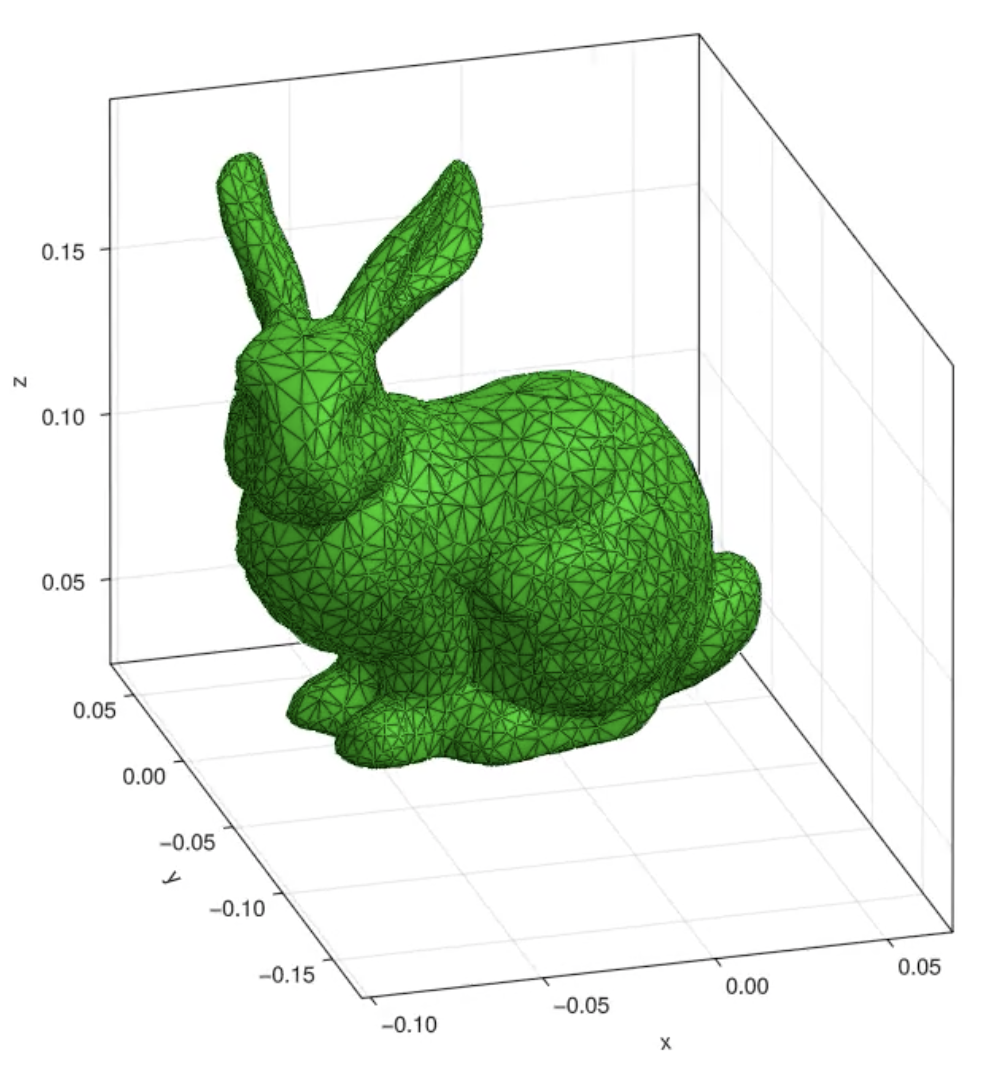
\includegraphics[width=\linewidth]{buni2.png}
\end{subfigure}
\begin{subfigure}{.4\textwidth}
  \centering
  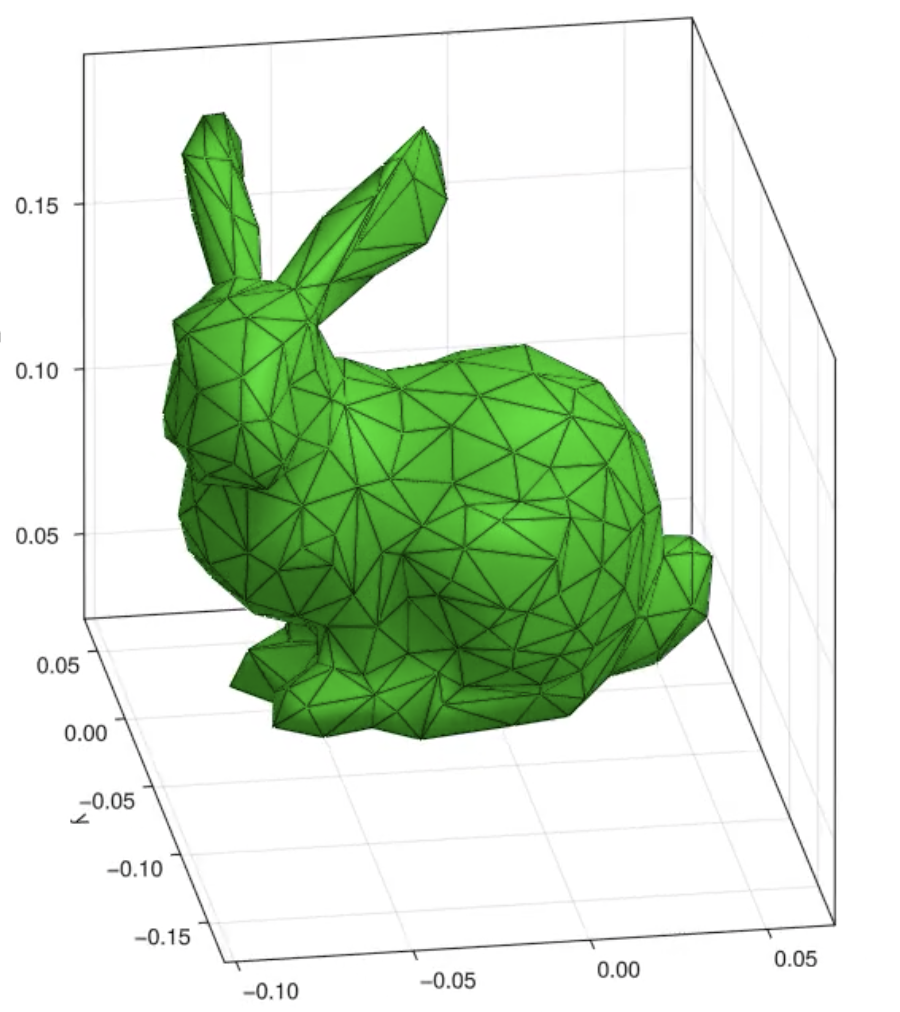
\includegraphics[width=\linewidth]{buni4.png}
\end{subfigure}
\begin{subfigure}{.4\textwidth}
  \centering
  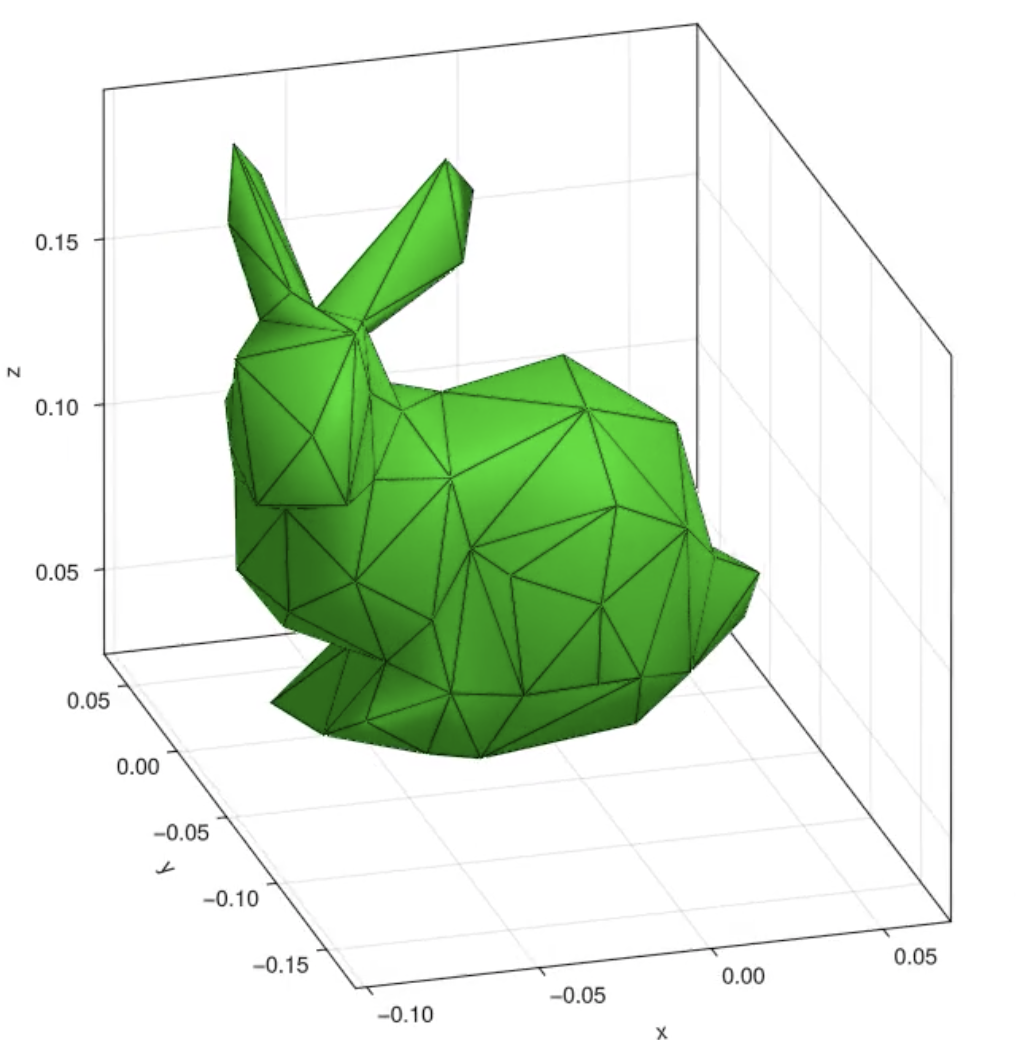
\includegraphics[width=\linewidth]{buni5.png}
\end{subfigure}
\caption{Contraction of the "Stanford Bunny" over time}
\end{figure}
\newpage
\item Motorcycle - https://www.artec3d.com/3d-models/motorbike?q=wage
\begin{figure}[h]
\centering
\begin{subfigure}{.4\textwidth}
  \centering
  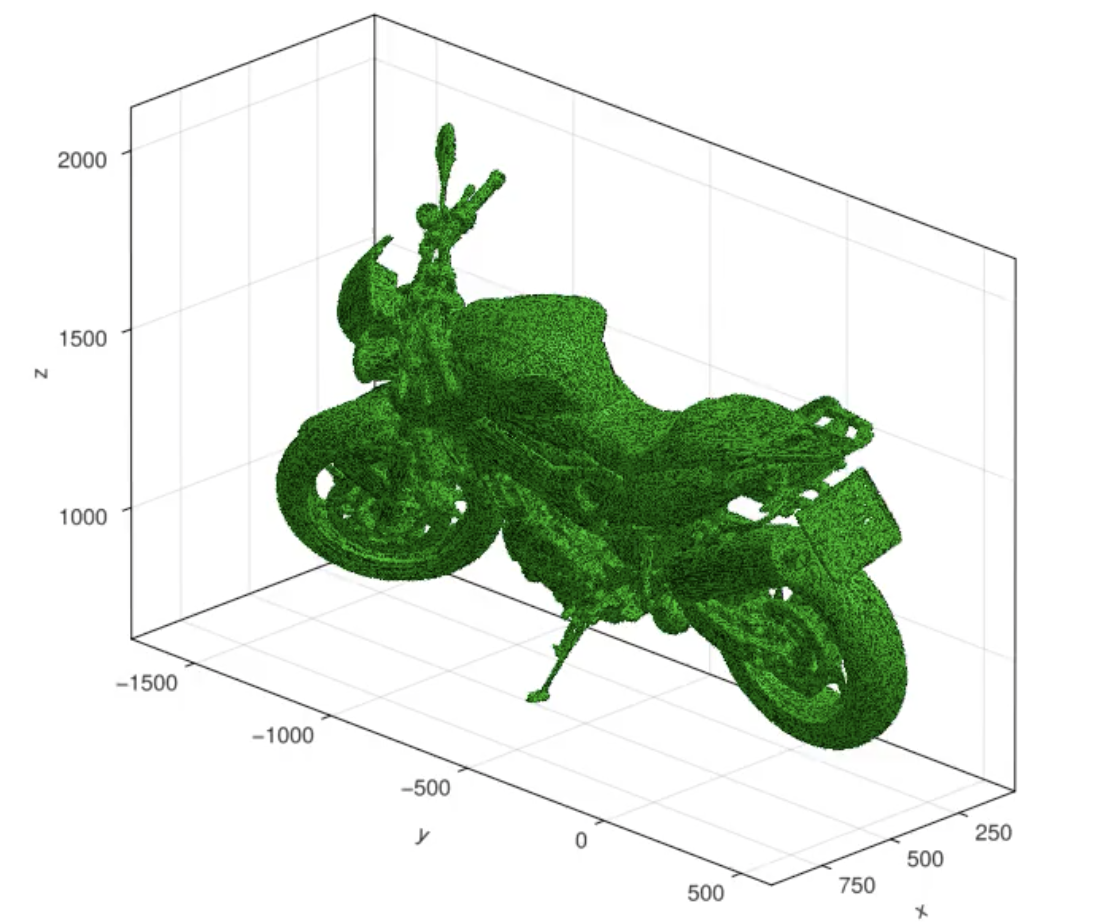
\includegraphics[width=\linewidth]{motorcycle1.png}
\end{subfigure}

\begin{subfigure}{.4\textwidth}
  \centering
  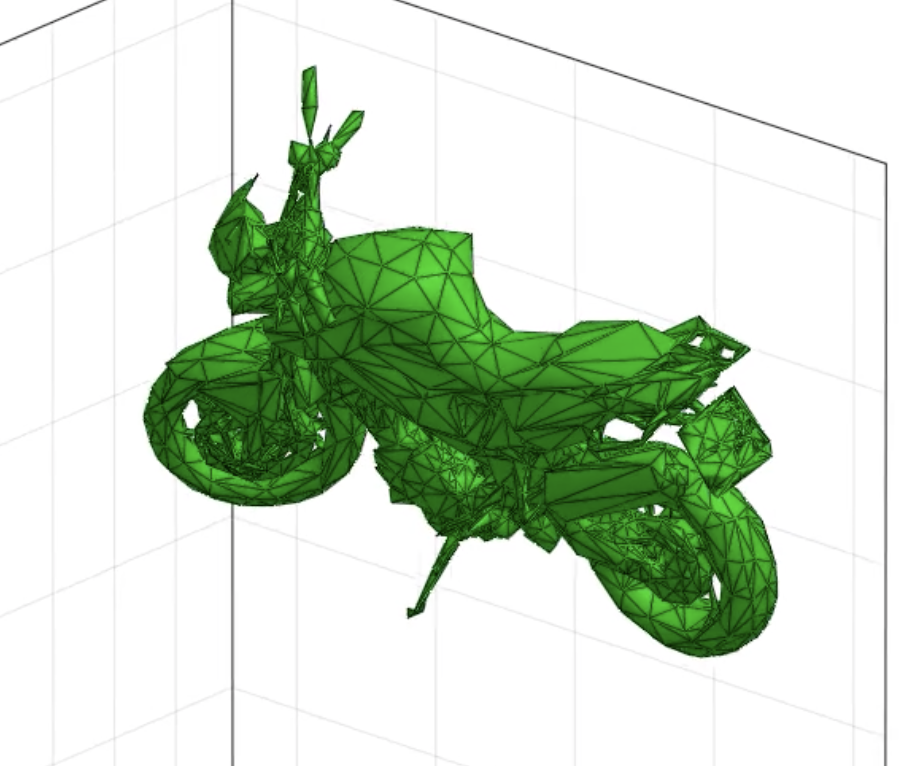
\includegraphics[width=\linewidth]{motorcycle5.png}
\end{subfigure}

\caption{Contraction of a 3D scanned motorcycle}
\end{figure}
\end{itemize}

As we can see from the images, the contraction algorithm greatly reduces the triangle count while preserving the shape, therefore the results met our expectations.
% References
\nocite{*}
\bibliography{references}
\end{document}